\documentclass[12pt]{book}
\usepackage[margin=.85in]{geometry} % for MARGIN
\usepackage[many]{tcolorbox}    	% for COLORED BOXES (tikz and xcolor included)


\usepackage{multicol}   
\usepackage{enumerate}
\usepackage[shortlabels]{enumitem}
\usepackage{varwidth}
\usepackage{tasks}
\usepackage[export]{adjustbox}
\usepackage[dvipsnames]{xcolor}

\usepackage{titleps}
\usepackage{setspace}               % for LINE SPACING
\usepackage[⟨options⟩]{fancyhdr}
\usepackage{enumitem}
\setlist{nosep}
\usepackage{tikz}
\usepackage{pgfplots}
\pgfplotsset{compat=1.5.1}
\usetikzlibrary{datavisualization}
\usetikzlibrary{datavisualization.formats.functions}

\newcommand{\D}{\displaystyle}


\setlength\parindent{0pt}   % killing indentation for all the text
\setstretch{1.3}            % setting line spacing to 1.3
\setlength\columnsep{0.25in} % setting length of column separator
\pagestyle{fancy}           % setting pagestyle to be headings

\usepackage[]{titlesec}

\fancyhead[L]{Math V04 - College Algebra}
\fancyhead[R]{Christina Papazacharioudakis}

\tcbset{
    sharp corners,
    colback = white,
    before skip = 0.2cm,    % add extra space before the box
    after skip = 0.5cm      % add extra space after the box
}                           % setting global options for tcolorbox

    \newtcolorbox{boxR}{
    fontupper = \color{black}, % font color
    boxrule = 1.5pt,
    colframe = black,
    rounded corners,
    arc = 5pt   % corners roundness
}

\definecolor{ballblue}{rgb}{0.13, 0.67, 0.8}

\begin{document}



\begin{comment}
Name: \underline{\hspace{100mm}}
\vspace{20mm}
  \centerline{\Large \textbf{Chapter 2: Equations and Inequalities} } 

{\large
\begin{center}
\begin{varwidth}{\textwidth}
\begin{enumerate}[2.1]
    \item The Regular Coordinate System and Graphs
    \item Linear Equations in One Variable
    \item Models and  Applications (Skipping)
    \item Complex Numbers
    \item Quadratic Equations
    \item Other Types of Equations
    \item Linear Inequalities and Absolute Value Inequalities
\end{enumerate}
\end{varwidth}
\end{center}

}
\newpage  
\end{comment}

\textbf{{\Large 3.5 \& 3.6 Transformations of Functions}}
\vspace{3mm}

Let's say we are asked to graph $g(x)=\sqrt[3]{x}+1$ or $g(x)= \sqrt[3]{x+1}$. Instead of making a table and plotting points, a method we can employ is to change or alter the toolkit function, $f(x)=\sqrt[3]{x}$ algebraically, and then make sense of those changes graphically. Let's started with how this process works.
\\

{ \large \textbf{Graphing Functions Using Vertical and Horizontal Shifts}}
\vspace{3mm}

\textbf{Identifying Vertical Shifts (Up and Down)}

One simple kind of transformation involves shifting a graph up or down. This upward and downward shift is called a \textbf{vertical shift}, because this involves adding a positive or negative constant to the function. 
\\

\begin{boxR}
    \textbf{Vertical Shift}
    \vspace{1mm}
    \hline 
    \vspace{2mm}

Given a function $f(x)$, a new function $g(x)=f(x)+k$ is a vertical shift of the function $f(x)$ by a constant value $k$.
\begin{itemize}
    \item If $k$ is positive, the graph will shift up.
    \item If $k$ is negative, the graph will shift down.
\end{itemize} 
\textcolor{BrickRed}{\emph{Observe that the vertical shift is a change happening outside of $f(x)$. That is, the change is happening outside of the parenthesis.}}
\end{boxR}




\centerline{\includegraphics[scale=1.3]{Chapter 3/3.5-figure1.jpeg}}

So if our goal is to graph \textcolor{Bittersweet}{$g(x) = f(x) +1$} and we only know what \textcolor{BlueViolet}{$f(x)$} looks like. We can start out with the graph of \textcolor{BlueViolet}{$f(x)$}, and shift the graph up by $1$.
\\


\newpage

\underline{\textbf{Example 1 - Adding a Constant to a function.}}

Graph $g(x) = x^2 + 3$ and $h(x)=x^2 - 1$ by identifying that $g(x)$ and $h(x)$ are vertical shifts to a toolkit function.


\vspace{10mm}


\begin{center}

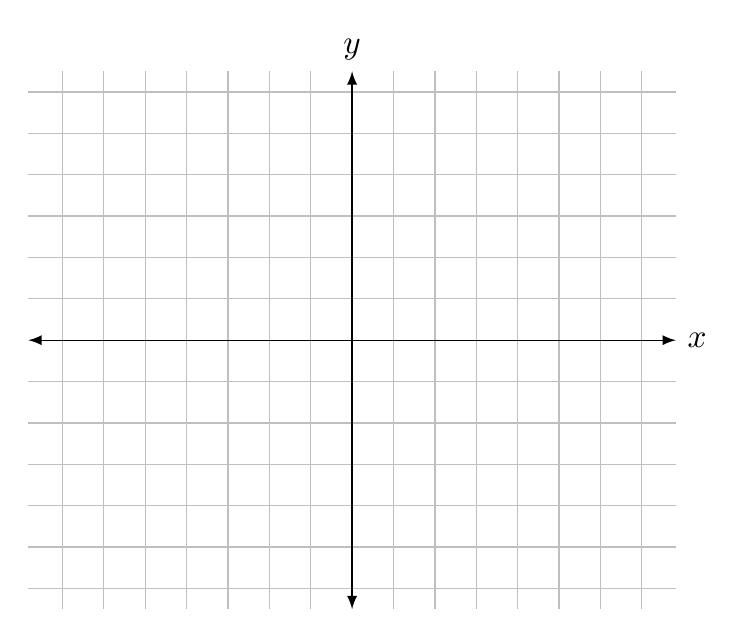
\begin{tikzpicture}[scale=1.2, transform shape]
\begin{axis}[
    ymin=-6.5,
    ymax=6.5,
    xmin=-6.5,
    xmax=6.5,
    axis on top=true,
    axis x line=middle,
    axis y line=middle,
    axis line style={latex-latex},
    xlabel=$x$,
    ylabel=$y$,
    xticklabels=\empty,
    yticklabels=\empty,
    xtick distance=1,
    ytick distance=1,
    xmajorgrids=true,
    ymajorgrids=true,
    axis equal = true, 
    every axis x label/.style={at={(ticklabel* cs:1.0)}, anchor=west,},
    every axis y label/.style={at={(ticklabel* cs:1.0)}, anchor=south,}
]
    \pgfplotsset{ticks=none}
\end{axis}
\end{tikzpicture}
\end{center}
\vspace{85mm}

\textcolor{BrickRed}{\emph{Observe that the vertical shift is a change happening outside of $x^2$}}

\newpage

{\textbf{Identifying Horizontal Shifts (Left and Right)}}

We just saw that the vertical shift is a change to outside of the function. We will now look at how changes on the inside of the function, and what this change means graphically. A shift to the input results in a movement of the graph of the function left or right in what is known as a \textbf{horizontal shift}.
\\

\begin{boxR}
    \textbf{Horizontal Shift}
    \vspace{1mm}
    \hline 
    \vspace{2mm}
Given a function $f(x)$, a new function $g(x)=f(x-h)$ is a \textbf{horizontal shift} of the function $f(x)$ by a constant value $h$.
\begin{itemize}
    \item If $h$ is positive, the graph will shift right.
    \item If $h$ is negative, the graph will shift left.
\end{itemize} 
\textcolor{BrickRed}{\emph{Observe that the horizontal shift is a change happening inside of $f(x)$. That is, the change is happening inside of the parenthesis.}}
\end{boxR}

\centerline{\includegraphics[scale=1.3]{Chapter 3/3.5-figure2.jpeg}}







So if our goal is to graph \textcolor{Bittersweet}{$g(x) = f(x+1)$} and we only know what \textcolor{BlueViolet}{$f(x)$} looks like. We can start out with the graph of \textcolor{BlueViolet}{$f(x)$}, and shift the graph up by $1$ to the left.
\\



\newpage

\underline{\textbf{Example 2 - Adding a Constant to the Input}}

Graph $g(x) = (x-1)^2$ and $h(x)=(x+3)^2$ by identifying that $g(x)$ and $h(x)$ are horizontal shifts to a toolkit function.

\vspace{5mm}
\begin{center}

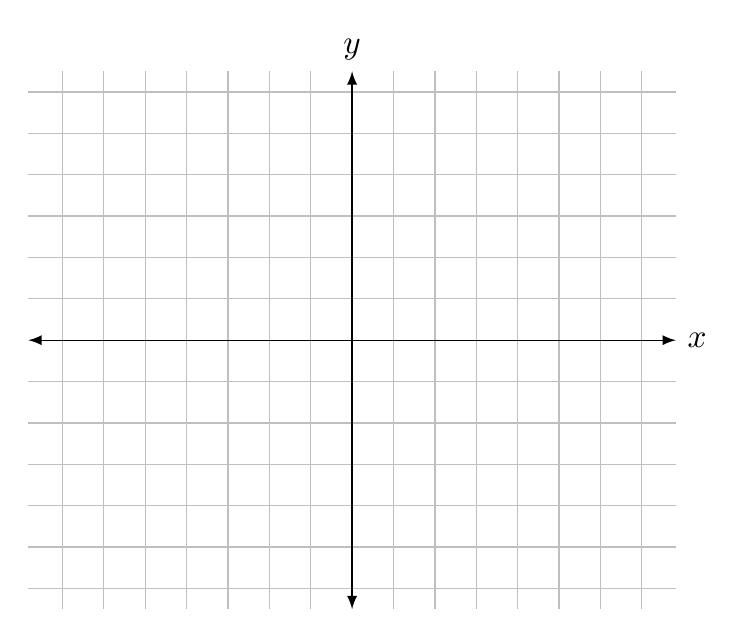
\begin{tikzpicture}[scale=1.2, transform shape]
\begin{axis}[
    ymin=-6.5,
    ymax=6.5,
    xmin=-6.5,
    xmax=6.5,
    axis on top=true,
    axis x line=middle,
    axis y line=middle,
    axis line style={latex-latex},
    xlabel=$x$,
    ylabel=$y$,
    xticklabels=\empty,
    yticklabels=\empty,
    xtick distance=1,
    ytick distance=1,
    xmajorgrids=true,
    ymajorgrids=true,
    axis equal = true, 
    every axis x label/.style={at={(ticklabel* cs:1.0)}, anchor=west,},
    every axis y label/.style={at={(ticklabel* cs:1.0)}, anchor=south,}
]
    \pgfplotsset{ticks=none}
\end{axis}
\end{tikzpicture}
\end{center}
\vspace{105mm}

\textcolor{BrickRed}{\emph{Observe that the horizontal shift is a change happening inside of $x^2$}}


\newpage


\underline{\textbf{Example 5 - Identifying a Horizontal Shift of a Toolkit Function}}
\vspace{3mm}


The following figure represents a transformation of the toolkit function $f(x)=x^2$. Relate this new function, $g(x)$ to $f(x)$, and then find the formula for $g(x)$.
\\


\centerline{\includegraphics[scale=1.3]{Chapter 3/3.5-figure3.jpeg}}


\newpage

\textbf{Combining Vertical and Horizontal Shifts}

Now that we have learned about two transformations, we can combine them. Vertical shifts are outside changes that affect the output (y-values) and shift the function up or down. Horizontal shifts are inside changes that affect the input (x-values) and shift the function left or right. Combining the two types of shifts will cause the graph of a function to shift up or down and left or right.
\\

\begin{boxR}
    \textbf{How To}
    \vspace{1mm}
    \hline
    \vspace{2mm}
\textbf{Given a function and both a vertical and a horizontal shift, sketch the graph.}

\begin{enumerate}
    \item Identify the vertical and horizontal shifts from the formula.
    \item The horizontal shift results from a constant added to the input. Move the graph left for a positive constant and right for a negative 
    \item The vertical shift results from a constant added to the output. Move the graph up for a positive constant and down for a negative constant.
constant.
    \item Apply the shifts to the graph in either order.
\end{enumerate}
\end{boxR}
\\

\underline{\textbf{Example 7 - Graphing Combined Vertical and Horizontal Shifts}}

Given $f(x) = |x|$, sketch the graph of $h(x)=f(x+1)-3$.
\vspace{20mm}
\begin{center}
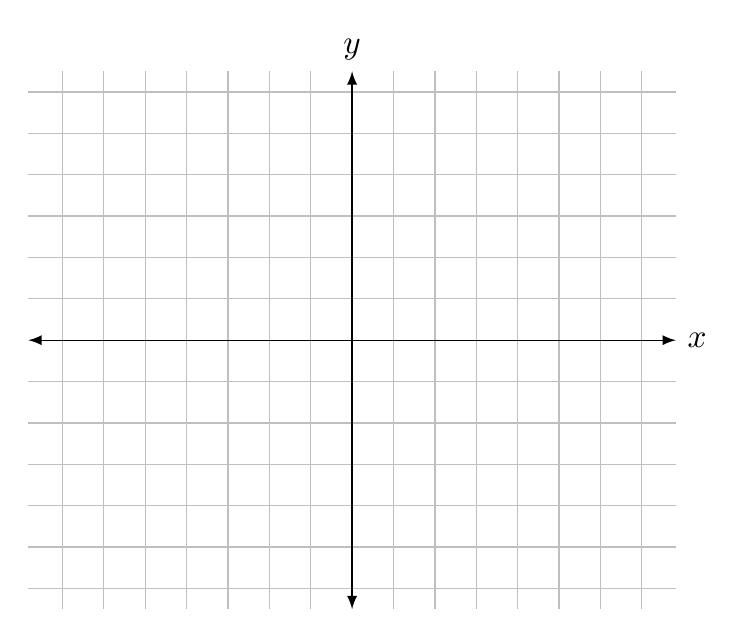
\begin{tikzpicture}[scale=1.2, transform shape]
\begin{axis}[
    ymin=-6.5,
    ymax=6.5,
    xmin=-6.5,
    xmax=6.5,
    axis on top=true,
    axis x line=middle,
    axis y line=middle,
    axis line style={latex-latex},
    xlabel=$x$,
    ylabel=$y$,
    xticklabels=\empty,
    yticklabels=\empty,
    xtick distance=1,
    ytick distance=1,
    xmajorgrids=true,
    ymajorgrids=true,
    axis equal = true, 
    every axis x label/.style={at={(ticklabel* cs:1.0)}, anchor=west,},
    every axis y label/.style={at={(ticklabel* cs:1.0)}, anchor=south,}
]
    \pgfplotsset{ticks=none}
\end{axis}
\end{tikzpicture}
\end{center}


\newpage
\underline{\textbf{Example 8 - Identifying Combined Vertical and Horizontal Shifts}}

Write a formula for the graph shown below, which is a transformation of the toolkit square root function.

\centerline{\includegraphics[scale=1.3]{Chapter 3/3.5-figure4.jpeg}}

\newpage
\textbf{Graphing Functions Using Reflections about the Axes}

Another transformation that can be applied to a function is a reflection over the x-axis or y-axis. A \textbf{vertical reflection} reflects a graph vertically across the x-axis. A horizontal reflection reflects a graph \textbf{horizontally} across the y-axis.

\centerline{\includegraphics[scale=1.3]{Chapter 3/3.5-figure6.jpeg}}

\vspace{5mm}

\begin{boxR}
    \textbf{Reflections}
    \vspace{1mm}
    \hline
    \vspace{2mm}
  Given a function $f(x)$, a new function $g(x)=-f(x)$ is a \textbf{vertical reflection} of the function $f(x)$. This is sometimes called a reflection over the $x-axis$

   Given a function $f(x)$, a new function $g(x)=f(-x)$ is a \textbf{horizontal reflection} of the function $f(x)$. This is sometimes called a reflection over the $y-axis$


\end{boxR}

\newpage

\begin{boxR}
    \textbf{How To}
    \vspace{1mm}
    \hline
    \vspace{2mm}
    \textbf{Given a function, reflect the graph both vertically and horizontally.}
    \begin{enumerate}
        \item Multiply all outputs by $–1$ for a \textbf{vertical reflection}. The new graph is a reflection of the original graph about the x-axis.
        \item Multiply all inputs by $–1$ for a \textbf{horizontal reflection}. The new graph is a reflection of the original graph about the y-axis.
    \end{enumerate}
\end{boxR}

\underline{\textbf{Example 8 - Reflect a Graph Horizontal and Vertically}}

Reflect the graph $s(t)= \sqrt{t}$ both \hspace{4mm} (a) Vertically (b) Horizontally


\newpage
{\large \textbf{Determining Even and Odd Functions}}

Some functions exhibit symmetry so that certain reflections result to the original graph.

\begin{boxR}
    \textbf{Even and Odd Functions}
    \vspace{1mm}
    \hline
    \vspace{2mm}
    \begin{itemize}
        \item  A function is called an \textbf{even function} if for every input $x$, 
    $$f(x)=f(-x)$$
    \textit{Applying a horizontal reflection results in the original graph}
    \item  A function is called an \textbf{odd function} if for every input $x$, 
    $$f(x)=-f(-x)$$
    \textit{Applying a horizontal reflection and a vertical reflection results in the same graph.}
    \end{itemize}
    
\end{boxR}

 \begin{boxR}
       \textbf{How To}
       \vspace{1mm}
       \hline 
       \vspace{2mm}
       \textbf{Given the formula for a function, determine if the function is even, odd, or neither.}
       \begin{enumerate}
           \item Determine whether the function satisfies $f(-x) = f(x)$.  If it does, it is even.
           \item Determine whether the function satisfies $-f(-x) = f(x)$.   If it does, it is odd.
           \item If the function does not satisfy either rule, it is neither even nor odd.
       \end{enumerate}
   \end{boxR}


\underline{\textbf{Example 12 - Determining whether a Function Is Even, Odd, or Neither}}

Determine if the function $f(x) = x^3 +2x$ is even, odd, or neither. 



\newpage
\textbf{{\large Graphing Functions Using Stretches and Compressions}}

Adding a constant to the inputs or outputs of a function changed the position of a graph (moving up, down, left, right), but it did not affect the shape of a graph. We now explore the effects of \textit{multiplying} the inputs or outputs by some quantity.
\\

\textbf{Vertical Stretches and Compressions}

When we multiply a function by a positive constant, we get a function whose graph is stretched or compressed vertically in relation to the graph of the original function.

\centerline{\includegraphics[scale=1.3]{Chapter 3/3.5-figure7.jpeg}}
\vspace{3mm}


\begin{boxR}
    Vertical Stretches and Compressions
    \vspace{1mm}
    \hline
    \vspace{2mm}
    Given a function $f(x)$, a new function $g(x)=a f(x)$, where $a$ is a constant, is a vertical stretch or vertical compression of the function $f(x)$
    \begin{itemize}
        \item If $a > 1$, then the graph will be stretched.
        \item If $a < 1$, then the graph will be compressed.
        \item If $a < 0$, then there will be combination of a vertical stretch or compression with a vertical reflection.
    \end{itemize}
\end{boxR}

\newpage

\underline{\textbf{Example 13 - Graphing a Vertical Stretch}}

A function $P(t)$ models the population of fruit flies. The graph is shown below. 

\centerline{\includegraphics[scale=1]{Chapter 3/3.5-figure8.jpeg}}

A scientist is comparing this population to another population, $Q(t)$,
whose growth follows the same pattern, but is twice as large. Sketch a graph of this population.
\vspace{35mm}


\underline{\textbf{Example 15 - Recognizing a Vertical Stretch}}

The graph below is a transformation of the toolkit function $f(x)=x^3$. Relate this new function, $g(x)$ to $f(x)$, and then find a formula for $g(x)$.
\\

\includegraphics[scale=1]{Chapter 3/3.5-figure9.jpeg}

\newpage

{\large \textbf{Horizontal Stretches and Compressions}}
Now we consider changes to the inside of a function. When we multiply a function’s input by a positive constant, we get a function whose graph is stretched or compressed horizontally in relation to the graph of the original function. If the constant is between 0 and 1, we get a \textbf{horizontal stretch}; if the constant is greater than 1, we get a \textbf{horizontal compression} of the function.
\\

\centerline{\includegraphics[sclae=1.3]{Chapter 3/3.5-figure10.jpeg}}
\vspace{3mm}

\begin{boxR}
    \textbf{Horizontal Stretches and Compressions}
    \vspace{1mm}
    \hline
    \vspace{2mm}
    Given a function $f(x)$, a new function $g(x)=f(bx)$, where $b$ is a constant, is a \textbf{horizontal stretch} or \textbf{horizontal compression} of the function.
    \begin{itemize}
        \item If $b > 1$, then the graph will be compressed by $b$
        \item If  $0<b<1$, then the graph will be stretched by $\frac{1}{b}$. 
        \item If $b <0$, then there will be combination of a horizontal stretch or compression with a horizontal reflection.
    \end{itemize}  
\end{boxR}


\newpage

\underline{\textbf{Example 18 - Recognizing a Horizontal Compression}}

Relate the function $g(x)$ to $f(x)$ in the following figure. 

\centerline{\includegraphics[scale=1.3]{Chapter 3/3.5-figure11.jpeg}}


\end{document}


